\chapter{Conclusion}
\label{chap:conclusion}
\section{Scope and Research Question}
This dissertation set out to interrogate a single guiding question: \textit{How does systematically reducing the \gls{flops} of a neural network influence its accuracy when exposed to radiation‑induced \gls{seu}?} 
In order to give the answer practical relevance for spacecraft designers who operate at opposite ends of the on‑board‐compute spectrum, the investigation adopted a deliberate two‑pronged scope. On the one hand, we examined a redundancy‑rich, decades‑old convolutional backbone VGG‑16 trained on the medium‑complexity CIFAR‑10 dataset. On the other, we analyses a purpose‑built, ultra‑compact classifier—CCDF\_MNIST whose parameter budget is compatible with sub‑watt micro‑controllers and whose target domain is the canonical MNIST digits. By juxtaposing those two archetypes we effectively spanned the range from flagship planetary probes equipped with multi‑watt FPGAs to pico and nano satellites that must make do with milliwatt‑class micro‑controllers. The resulting design space therefore reflects the heterogeneous reality of modern space missions and guarantees that the proposed rule‑of‑thumbs are not tied to a single hardware tier.








\section{Method Synopsis}

Our methodology comprises four synergistic stages as depicted in Figure~\ref{fig:method_flow}:
\label{sec:method}
To chart that space we chained four optimization and evaluation steps into a single workflow. First, we applied iterative, L1‑norm structured pruning to remove entire filters or channels in gradually increasing fractions. Constraining the per‑iteration pruning ratio by
\[
r_t = \min\!\bigl(0.2\,\bigl(1+0.1t\bigr),\,0.5\bigr)
\]
ensured that the network could settle into a new optimum before the subsequent pruning round was initiated, thereby avoiding catastrophic capacity cliffs. Second, we compressed both weights and activations to signed‑integer ranges through 8‑bit post‑training quantitation, harvesting an additional four‑fold reduction in model memory footprint and, by extension, SRAM upset cross‑section. Third, we replicated the radiation environment by means of the QSEU injector, which flips random bits inside quantized weight tensors in direct proportion to the model’s live \gls{flops},this simulate the errors occurred when \gls{flops} is changing. Finally, after every pruning stage we performed short cycles of fine‑tuning under a cosine‑annealed stochastic‑gradient‑descent schedule to claw back as much nominal accuracy as possible before the next round of structural compression.



\begin{figure}[H]
    \centering
    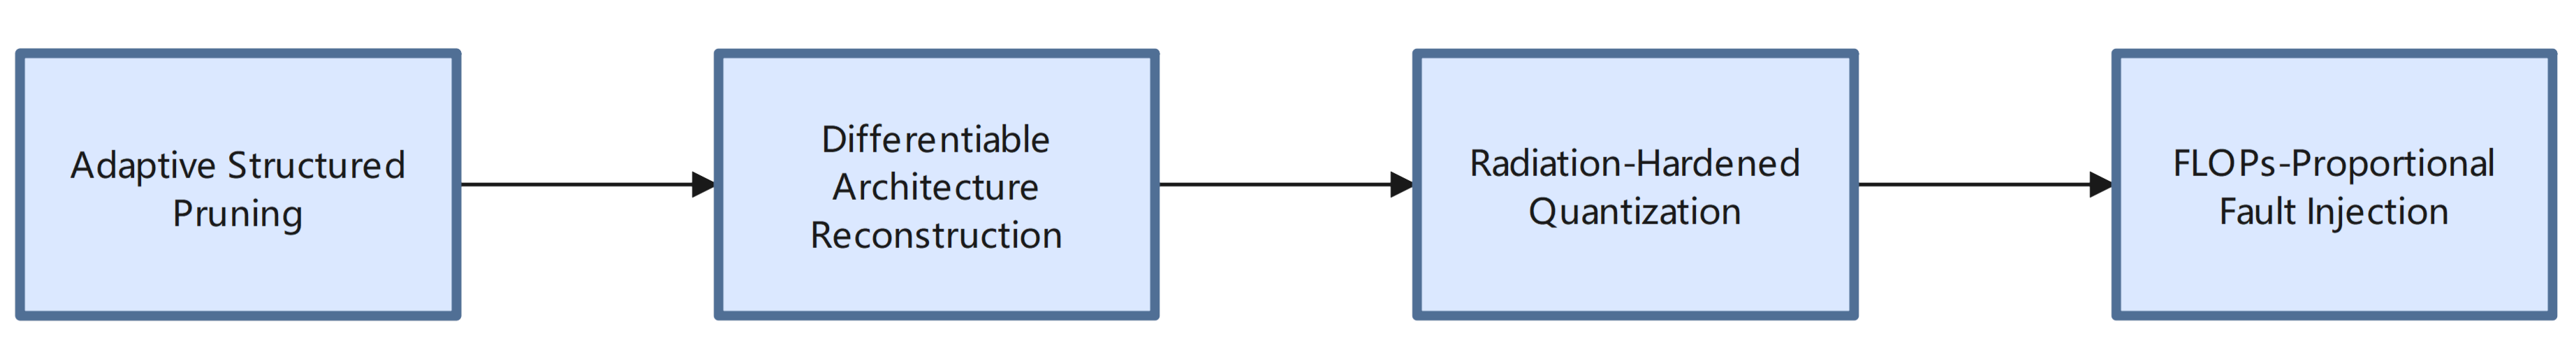
\includegraphics[width=1\linewidth]{images/FLOW.png}
    \caption{Overview of the proposed robustness evaluation pipeline. 
    The workflow consists of: (1) iterative structured pruning based on L1-norm filter ranking, 
    (2) post-training quantization using 8-bit affine mapping, 
    (3) fault injection proportional to model \gls{flops} using the QSEU framework to simulate realistic bit-level errors, and 
    (4) fine-tuning with cosine annealing to mitigate the impact of compression and faults. 
    This pipeline is designed to evaluate model robustness under fault injection scenarios rather than radiation-hardening contexts.}
    \label{fig:method_flow}
\end{figure}









\section{Key Findings}
The large VGG‑16 baseline proved remarkably forgiving. After ten pruning‑and‑retraining rounds the network’s computational load had fallen from 229.05M to 43.38M \gls{flops}, an 86\% reduction, yet its clean‑room accuracy dropped by merely 3.7\%. Under fault injection the total degradation grew to 5.1 percentage points. The result corroborates the intuition articulated by Catalan \cite{Catalan2025} that modern convolutional architectures possess ample representational slack and that their inherent redundancy masks isolated bit flips almost for free. 

The compact \texttt{CCDF\_MNIST} model, by contrast, behaved in line with its frugal parameter count. Pruning 71\,\% of its 0.42\,M \gls{flops} incurred only a modest 2.9\,pp accuracy hit in the absence of faults but amplified the SEU‑induced loss to a steep 20.4\,pp. That observation echoes the findings of Nazemi \cite{Nazemi2021}, who warned that aggressively compressed classifiers lose the combinational diversity required to re‑route information around corrupt weights. 

Taken together, the experiments invite a pragmatic design heuristic: generously‑sized convolutional backbones can tolerate on the order of 50\,\% structured pruning before their radiation robustness starts to erode markedly, whereas highly optimised, bespoke models should remain below roughly 30\,\% pruning unless augmented by external error‑correcting codes.










\section{Limitations}
While the workflow delivered reproducible \gls{flops}–robustness curves, three caveats delimit its external validity. 
First, the fault model was intentionally simplified; only temporally and spatially independent single‑bit upsets were simulated. In reality, heavy‑ion tracks often cause multi‑bit upsets or even latch‑ups that disable complete memory banks. Without modeling those correlated events, the present study may over‑estimate achievable robustness. 
Second, the architectural breadth was narrow. The experiments focused on a single convolutional family and one bespoke miniature network. Whether the conclusions transfer to attention‑centric vision transformers, multi‑sensor fusion networks, or neuromorphic spiking nets remains an open question. 
Third, the hardware loop was closed only by extrapolation. All timing and energy figures were measured on NVIDIA GPUs and then projected onto rad‑hard processors such as the GR740. The lack of hardware‑in‑the‑loop validation leaves room for secondary effects—e.g.\ cache contention or bus stalls—that could shift the Pareto front in practice.










\section{Impact}
Despite those limitations, the dissertation makes a concrete contribution to the field of radiation‑tolerant artificial intelligence. For the first time, engineers are offered quantitatively derived \gls{flops}–robustness curves rather than anecdotal estimates. The curves allow mission planners to trade margin against mass: a rover architect can now ask how many extra grams of battery he must budget to gain a specific safety buffer in classification accuracy, or inversely, how much accuracy he is prepared to sacrifice in exchange for a lighter launch payload. The study thus complements classical hardware‑centric hardening techniques—triple‑modular redundancy, body biasing, silicon‑on‑insulator—with a software‑centric knob whose cost can be dialed in fine increments.










\section{Future Work}
In future work, we aim to enhance the statistical rigor of our evaluation by adopting a Monte Carlo-style sampling procedure. This will include multiple runs across varying random seeds, randomized fault maps, and diverse model initializations, enabling the computation of standard deviations and 95\% confidence intervals. Such an approach will support more robust statistical comparisons and hypothesis testing.

Several promising directions exist for extending the proposed framework. A natural next step is to incorporate correlated fault simulators that account for spatial multi-bit upsets and temporal burst errors—ideally validated through heavy-ion beam experiments. Another compelling avenue involves exploring attention-based and hybrid CNN–Transformer architectures, as their self-attention mechanisms may exhibit distinct redundancy properties, thereby affecting the trade-off between pruning and robustness.









\section{Final Remarks}
In summary, this work demonstrates that moderate, structure‑aware pruning of over‑parameterized convolutional networks constitutes a potent first‑line defense against radiation faults in space‑borne machine‑vision systems. By quantifying the trade‑offs between computational economy and fault resilience with unprecedented granularity, the thesis lays the empirical foundation for a new generation of resource‑aware, autonomous spacecraft. Over the next decade, as exploration missions venture farther and operate with ever less ground support, such software‑level hardening will become an indispensable complement—not a replacement, but a peer—to conventional electronic countermeasures.\par
Ultimately, the line of enquiry opened here points towards a unifying principle: robustness is not a binary property conferred by a single shield or algorithm, but a spectrum along which compute, energy, and accuracy can be finely negotiated. The charts and findings presented in these pages offer mission engineers the quantitative vocabulary to conduct that negotiation with confidence.